\subsection{State Charts}

\subsubsection{Daily Plan State Diagram}
This state diagram shows the three states of a Daily Plan.\\
The Daily Plan is \textit{Created} by the system and then \textit{Updated} or carried out and \textit{Confirmed} by the agronomist, depending on whether he needs to change the plan or not.
\begin{figure}[h!]
  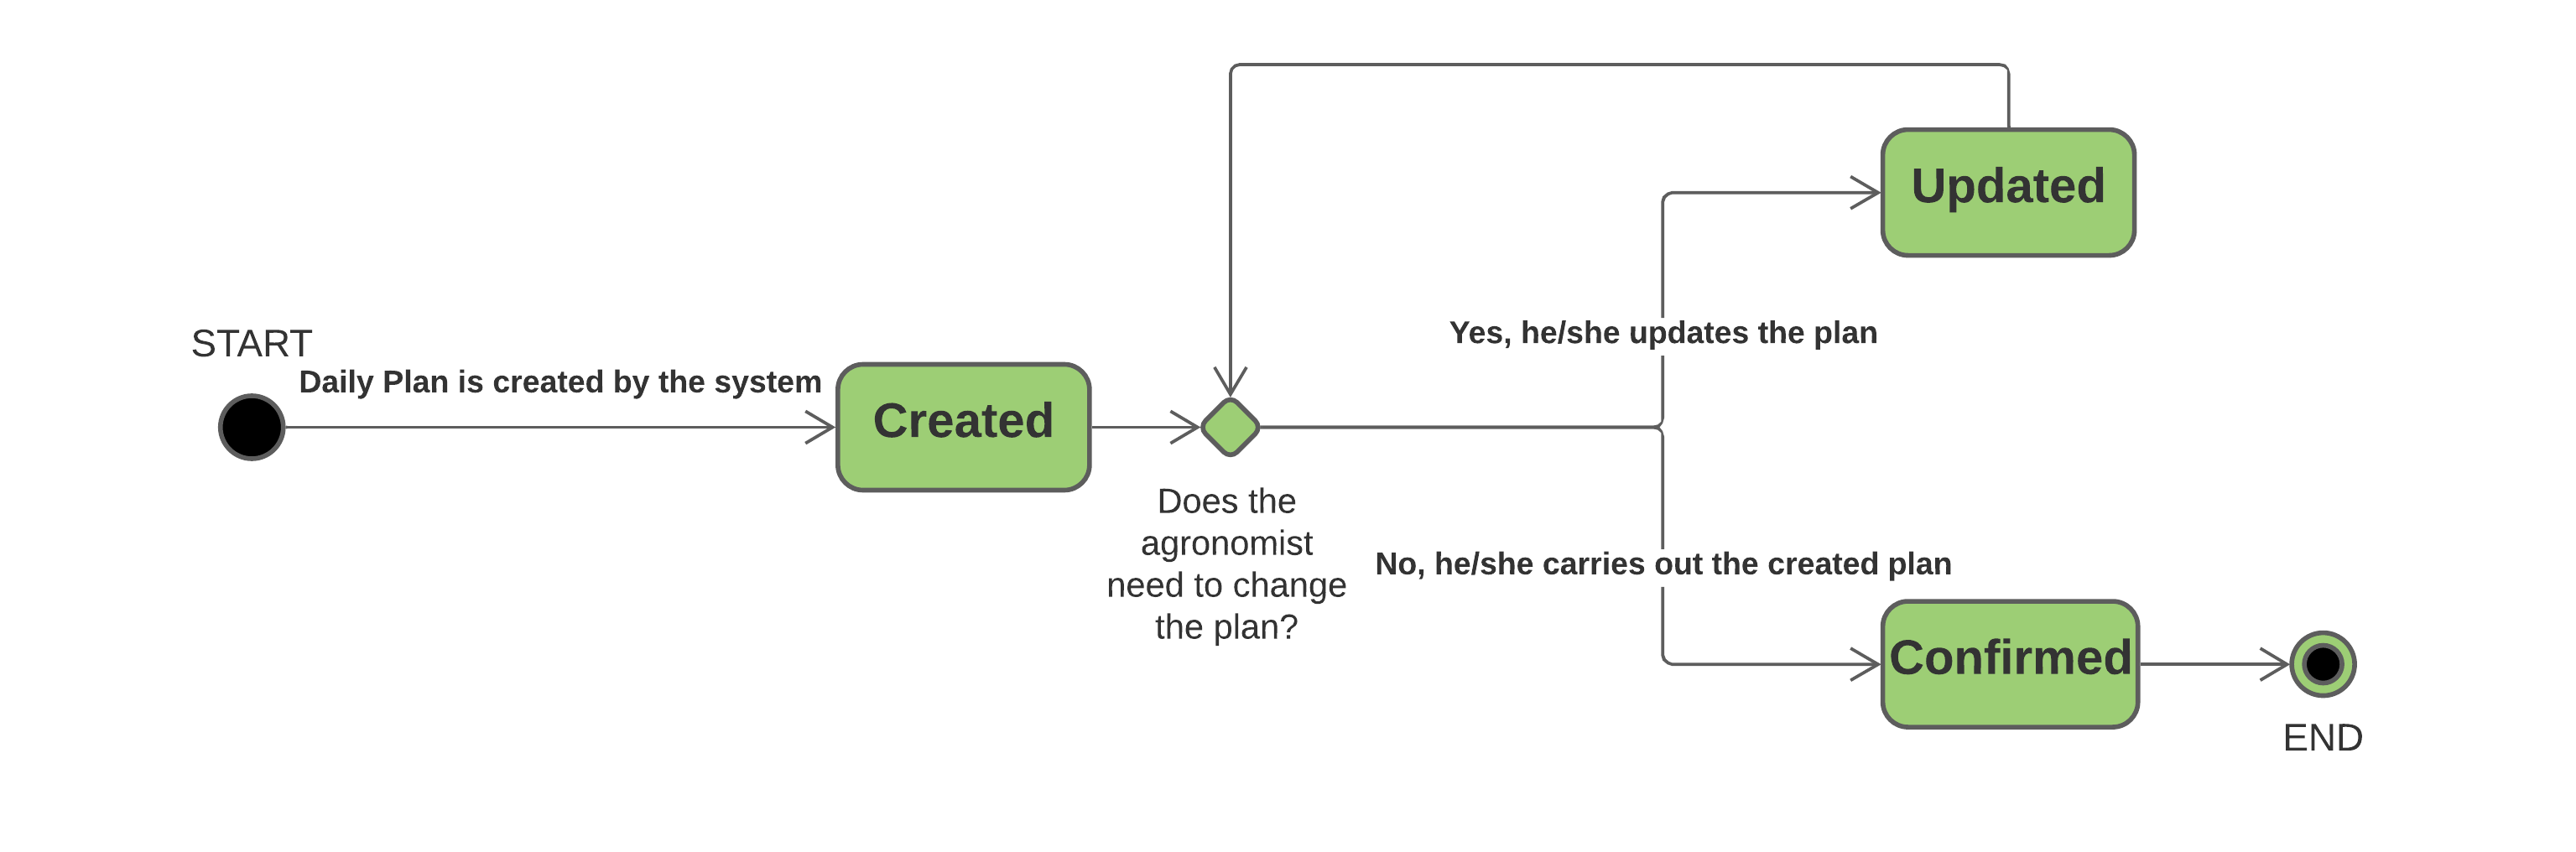
\includegraphics[width=\textwidth,height=\textheight,keepaspectratio]{./Images/State Chart DailyPlan.png}
  \caption{Daily Plan State Diagram}
\end{figure}

\subsubsection{Help Request State Diagram}
This state diagram shows the two states of a Help Request.\\
The Help Request is \textit{Created} and then \textit{Solved} by the farmer, depending on whether he is satisfied with the reply received or not.
\begin{figure}[h!]
  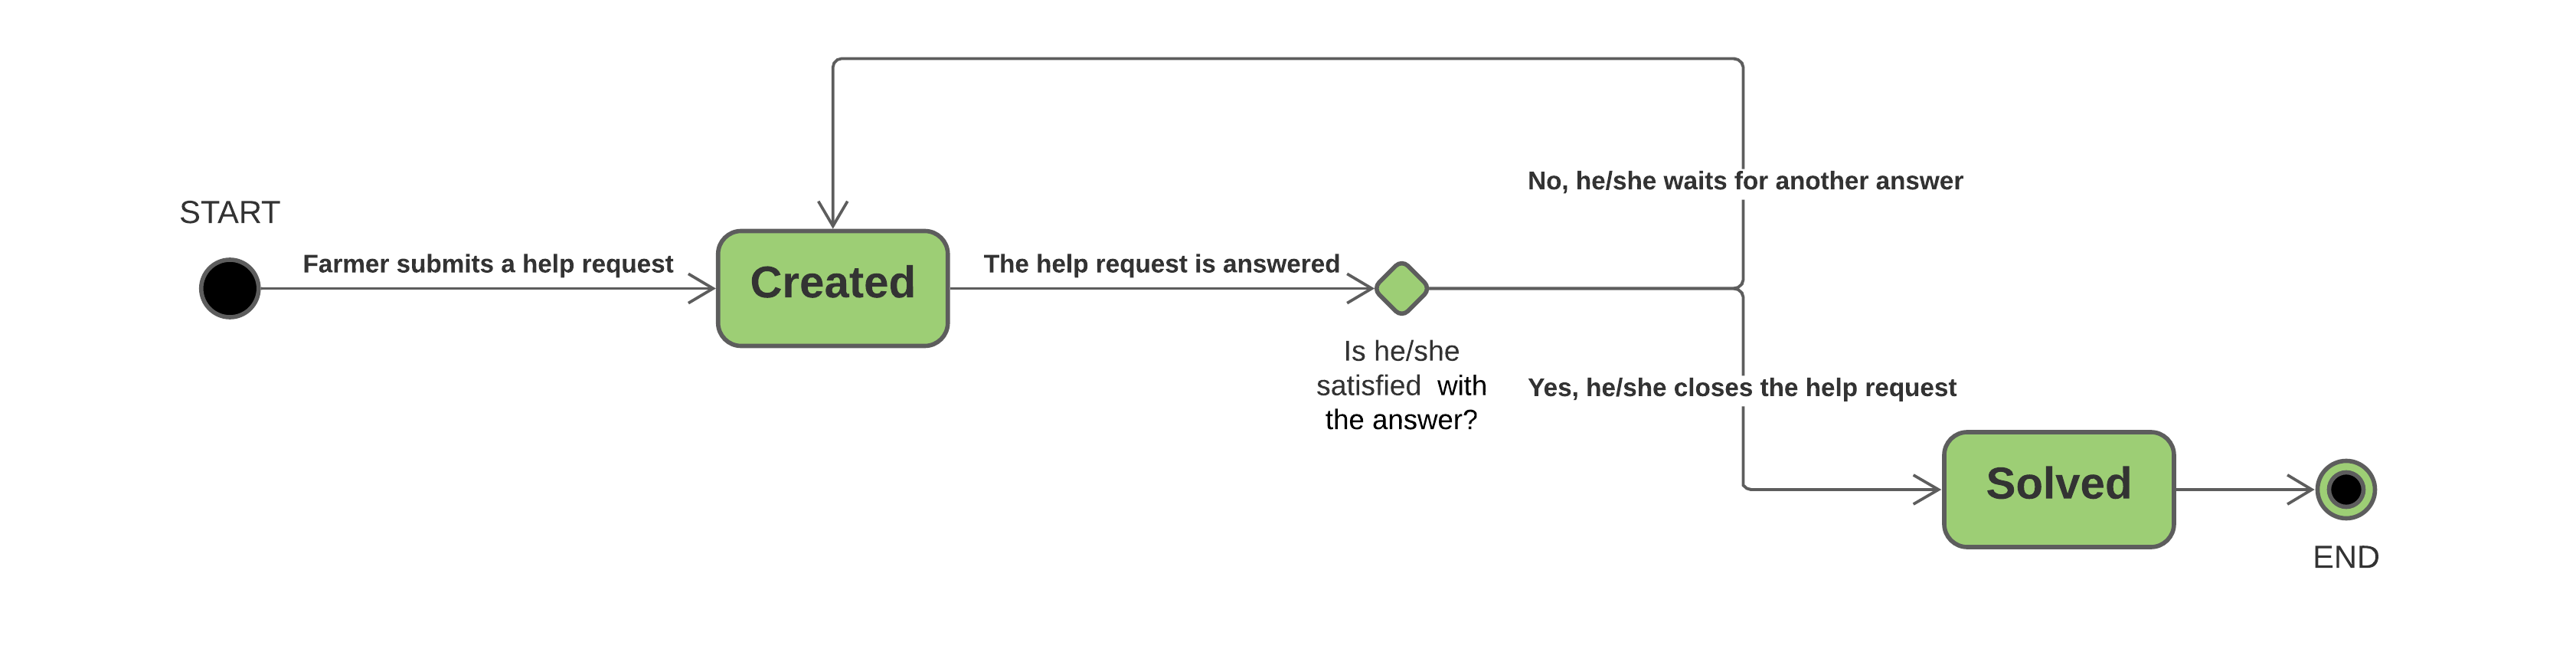
\includegraphics[width=\textwidth,height=\textheight,keepaspectratio]{./Images/State Chart HelpRequest.png}
  \caption{Help Request State Diagram}
\end{figure}

\subsubsection{Discussion Forum State Diagram}
This state diagram shows the two states of a Discussion Forum.\\
The Discussion Forum is \textit{Created} and then \textit{Solved} by the farmer, depending on whether he is satisfied with the replies received or not.
\begin{figure}[h!]
  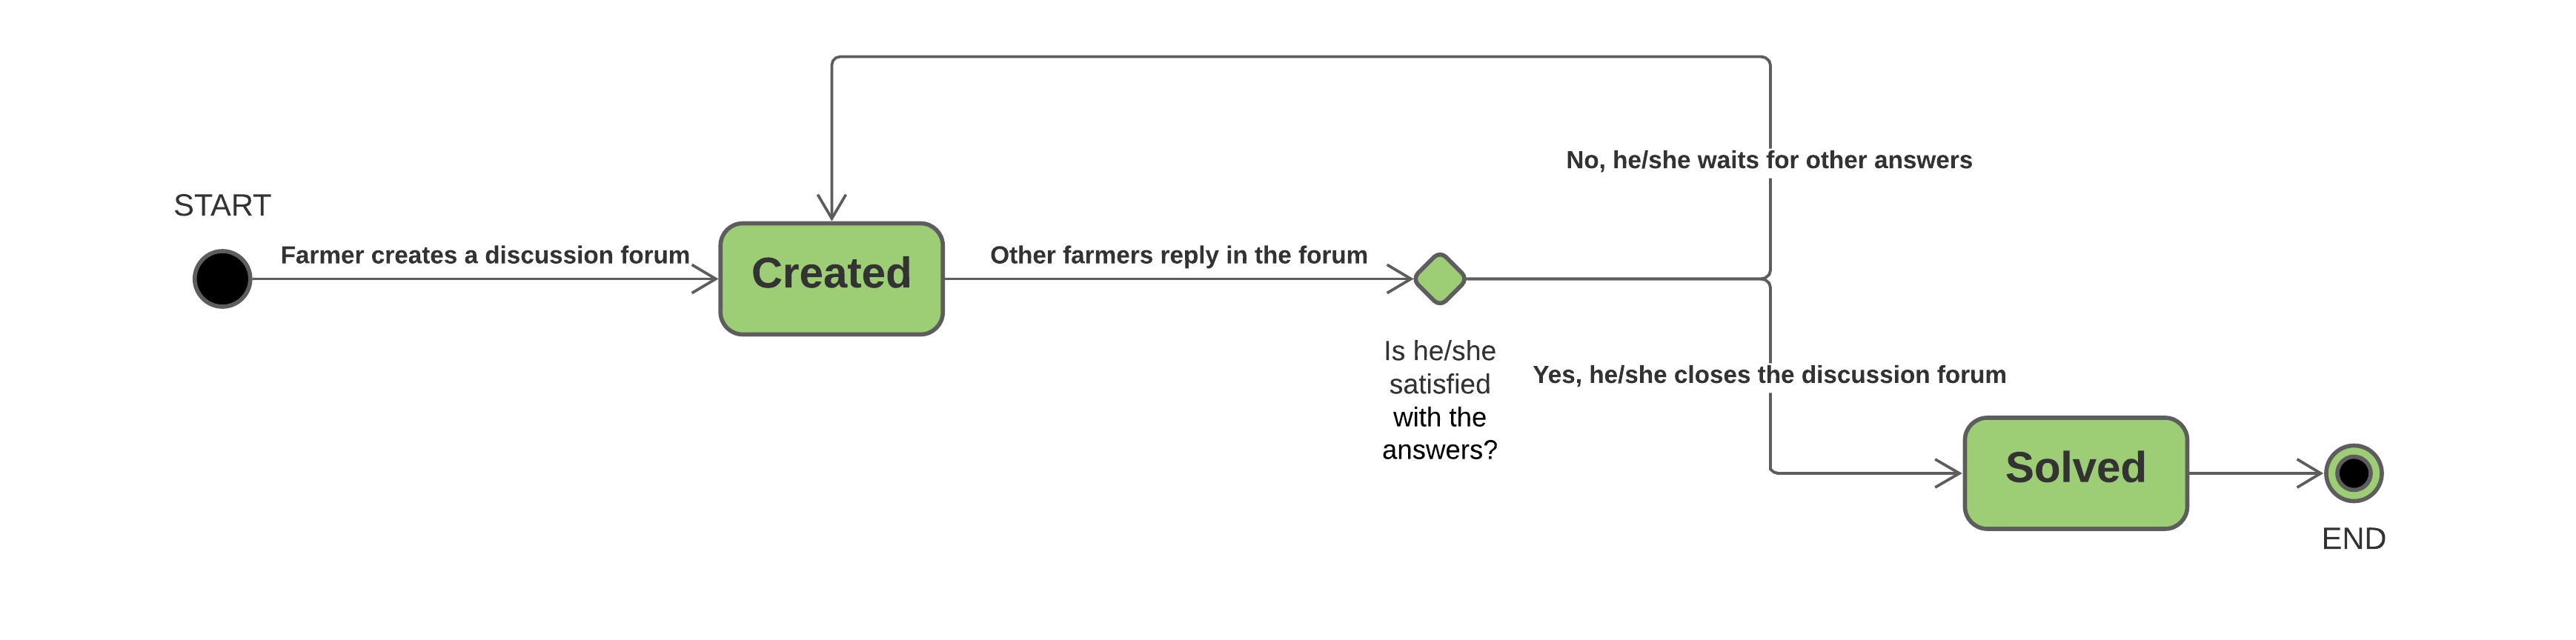
\includegraphics[width=\textwidth,height=\textheight,keepaspectratio]{./Images/State Chart DiscussionForum.png}
  \caption{Discussion Forum State Diagram}
\end{figure}

\subsubsection{Visit State Diagram}
This state diagram shows the two states of a Visit.\\
The Visit is \textit{Scheduled} and then \textit{Done} after the agronomist carries out the visit and confirms the corresponding Daily Plan.
\begin{figure}[h!]
  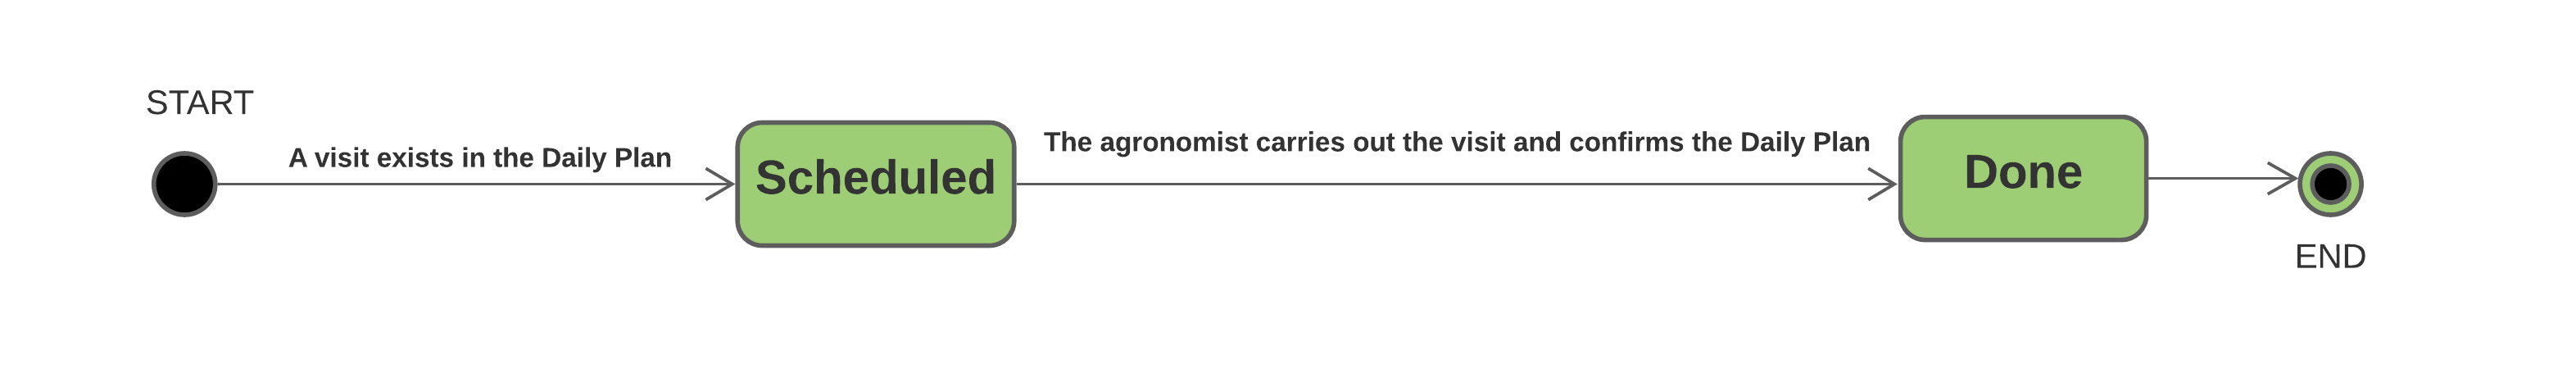
\includegraphics[width=\textwidth,height=\textheight,keepaspectratio]{./Images/State Chart Visit.png}
  \caption{Visit State Diagram}
\end{figure}
